\begin{abstract}
Target-cell conditioning in arbitrary-scale super-resolution can improve
average reconstruction while harming particular images or frequency bands.
We investigate this discrepancy using saved natural-image outputs and
controlled probes of frozen models. Low-resolution Nyquist normalisation
reduces cross-scale recovery variation in all 27 model--dataset--seed
groups, but pooled consistency hides image-wise differences. An exact
squared-error decomposition separates harmful corrections into overshoot
and wrong direction: their frequencies differ between LTE and SC-INR and
between band and full-RGB evaluation. Halving the correction rescues
11/13 and 6/27 harmful band outcomes, respectively, yet increases overall
RGB MSE by 2.41\% and 0.97\%. At fixed scale, controlled high-frequency
input paths can reverse correction alignment; changing target phase at
fixed power also reverses readout gain. These finite experiments show
why frequency ordering and global attenuation are insufficient descriptions
of readout benefit. They provide conditional failure diagnostics, rather
than a new decoder, a deployable selector or a universal causal mechanism.
\end{abstract}
\begin{keywords}
Arbitrary-scale super-resolution, cell conditioning, frequency recovery,
readout failure analysis
\end{keywords}

\section{Introduction and Related Work}
\label{sec:intro}
Arbitrary-scale super-resolution (ASISR) predicts image values at continuous
coordinates. LIIF supplies target cell size to a local decoder
\cite{chen2021liif}; LTE introduces cell-dependent phase estimation
\cite{lee2022lte}. This information specifies the requested scale but does
not guarantee that the resulting output change reduces reconstruction
error. Our question is: \emph{at the same scale and frequency band, why
can a cell-conditioned correction help one image and hurt another?}
We examine output-level failure types and controlled conditions that
change benefit, without identifying an internal neural mechanism.

Harmful cell effects are not new. LIIF already varies cell size at fixed
queries; IPE-LIIF integrates positional features and reports cases where
an additional cell input hurts \cite{liu2021ipe}. Thera supplies analytic
Gaussian filtering and discusses its mismatch with bicubic training
\cite{becker2025thera}. Our fixed-checkpoint interventions are not a
performance comparison against these methods. Integrating intermediate
features also need not equal integrating a nonlinear decoder's RGB output.

Frequency-resolved analysis has precedents in HyRA's linear/nonlinear
responses \cite{fsds2024}, texture-based error analysis
\cite{magid2022texture}, sinusoidal degradation probes
\cite{kawai2026frequency}, and Nyquist-normalised forecasting
\cite{wang2026scaleanchoring}. The importance of phase beyond spectral
magnitude is classical \cite{oppenheim1981phase}. We do not claim these
principles, or the quadratic identity below, as new. A wider continuous-SR
benchmark studies architecture and retraining effects
\cite{nasir2026empirical}; we isolate interventions on inherited models.

Our contribution is a connected empirical diagnosis. First, we establish
a useful frequency coordinate while showing how pooling conceals
image-wise variation. Second, we distinguish overshoot from wrong-direction
corrections, quantify their different band/RGB consequences, and test
high-frequency input paths and phase at fixed scale. These controls locate
conditions missing from coarse spectral descriptions. Failed observation-only
forecasts remain evidence of a gap between explanation and decision,
and are evaluated separately from the descriptive findings.

\section{Evaluation Objects and Frequency Recovery}
\label{sec:recovery}
\subsection{Keep the comparison fixed}
Let $y=Ax$ denote the LR observation, $Q_hx$ the desired target measurement,
and $c$ the cell supplied to $F_\theta(y,q,c)$. Changes to $A$, $Q_h$ and
$c$ answer different questions. Natural-image tests use discrete HR targets
and bicubic antialiased downsampling, not certified box averages of a
known continuous field. Assigning $c=h$ does not establish that the model
implements the physical operator $Q_h$.

The LIIF/LTE/SC-INR variants inherit an EDSR-baseline encoder, DIV2K
training \cite{agustsson2017div2k}, 1000 epochs and training scales
$\times1$--$\times4$. SC-INR is the examined sinc-modulated Fourier-feature
implementation. A trained full/no-readout ablation changes weights;
a native/zero-cell comparison holds weights, observation and queries
fixed. Zero cell may be outside training support. Frozen probes use one
seed1 checkpoint per LTE/SC model; this LTE snapshot omits the original
paper's extrapolation cell clamp. Claims concern these implementations.

\subsection{A useful coordinate with image-wise exceptions}
For image $i$, band $b$, target energy $S_{ib}=\|\Pi_b(x_i-\bar x_i)\|^2$
and error energy $E_{ib}=\|\Pi_b(x_i-\hat x_i)\|^2$, define
\begin{equation}
\begin{aligned}
 R_b&=1-\frac{\sum_i E_{ib}}{\sum_i S_{ib}},\\
 D&=\operatorname{median}_b[\max_s R_b(s)-\min_s R_b(s)].
\end{aligned}
 \label{eq:recovery}
\end{equation}
The frequency study uses the RGB mean, unwindowed FFTs, centre HR240
crops and respectively 14, 30 and 30 images from Set14, BSD100 and Urban100
\cite{zeyde2010single,martin2001database,huang2015urban}. With Chebyshev
frequency $\nu=\max(|\nu_x|,|\nu_y|)$ and scale $s=2,3,4$, seven bins
span $.25,.5,\ldots,2$ in $u=2s\nu$; $u=1$ is LR Nyquist. The absolute
control fixes bin edges at $\nu=u/6$. Different bin supports compare
evaluation coordinates, not equality of reconstructed functions.

Normalisation reduces $D$ in all nine primary model--dataset groups,
from $.31$--$.46$ to $.013$--$.061$, and all 27 groups including two
additional seeds. The original requirement of $D\le.05$ in eight of
nine primary groups fails (6/9). In 24 saved-output sensitivity settings
covering frequency subdomains, scale pairs and pooling, all 27 groups
retain the reduction; these are dependent comparisons. On the original
domain, the tolerance passes 19/27 pooled versus 27/27 equal-image groups.

To separate weighting from image-wise changes, write
$R_{sb}=\sum_iw_{isb}R_{isb}$ with $w_{isb}=S_{isb}/\sum_jS_{jsb}$.
Holding weights at $\bar w_{ib}=\frac13\sum_sw_{isb}$ reduces $D$ in all
nine Set14 groups ($.0493$--$.0616$ to $.0227$--$.0294$) but increases it
in all nine Urban100 groups ($.0147$--$.0202$ to $.0293$--$.0538$).
All nine Urban100 pooled curves pass $.05$, while only 14--17 of 30
individual images per group pass that same descriptive tolerance.
Weights can amplify or conceal variation; HR-dependent reweighting is
neither a deployable rule nor an independently identified physical cause.

\begin{figure*}[t]
\centering
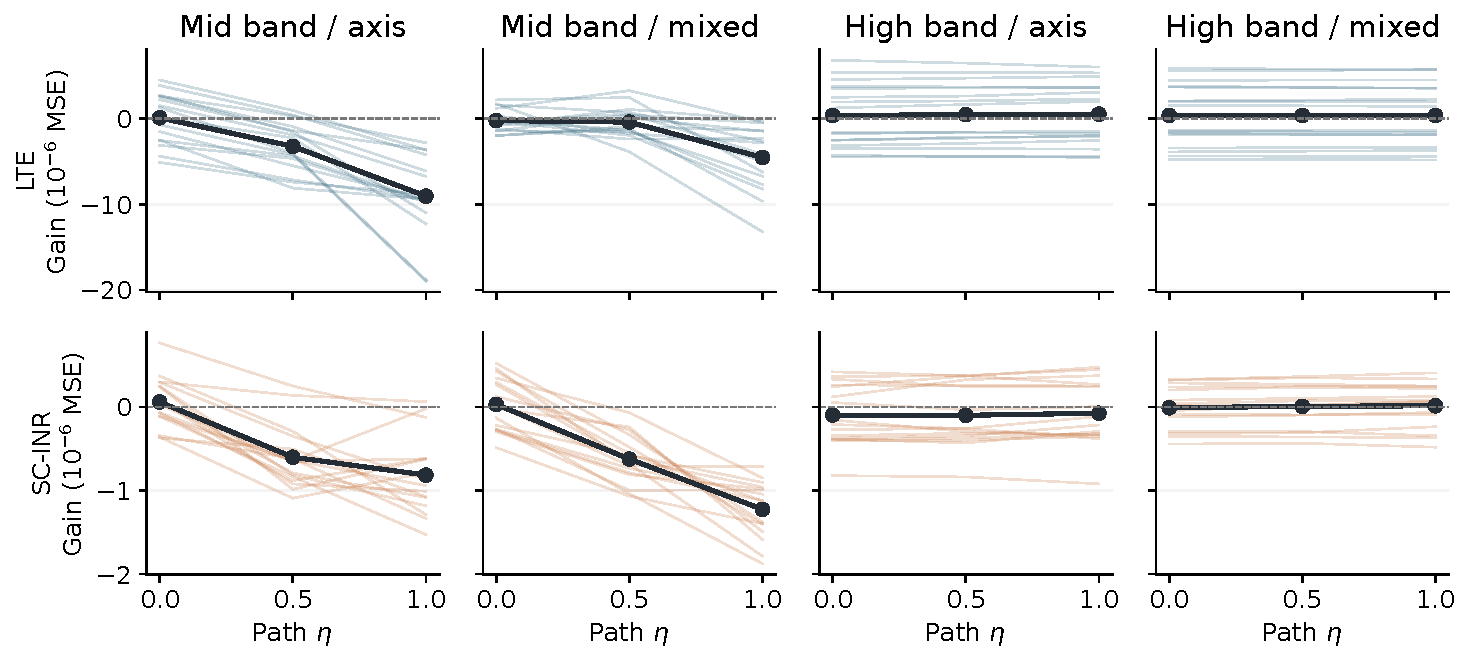
\includegraphics[width=.95\textwidth]{figures/icassp-controlled.pdf}
\caption{All phase/position conditions of the four supra-Nyquist templates
(primary centre32 region). Thin lines show 16 related phase--position
conditions per panel; dark lines are finite-grid means, not confidence
intervals. Columns 1--2 measure middle-band gain, columns 3--4 high-band
gain, in $10^{-6}$ MSE units. Negative values mean native cell is worse
than zero cell. These relative readout gains are not total reconstruction
quality changes under the input-path intervention.}
\label{fig:controlled}
\end{figure*}

\section{From Frequency Ordering to Failure Types}
\label{sec:failure}
\subsection{Coarse ordering is an insufficient explanation}
In LTE/SC seeds 2 and 3, trained full/no-readout recovery
losses meet the frozen band-order criterion ($\rho\ge.5$); high-band loss
exceeds middle-band loss in 34/36 dataset--scale settings. Yet the
footprint score $(.00006,.00552,.07235)$ has exactly the same ranks as
band index $(1,2,3)$. These paired tests use RGB-mean HR256 crops and
three bands cut at $1/8,1/4,1/2$. A separate HR240 test averages full-model
outputs over 31 conditioning scales $1,1.1,\ldots,4$ at fixed features
and queries. Its ordering passes the separate ordering criterion
($\rho\ge.7$) in 4/4 groups, but passes its $.8$ function-similarity
criterion in 0/4 and exceeds the matched footprint correlation by $.05$
in only 2/4. Similarity is the fraction of cases where the trained
ablation is closer to the averaged than to the full output. Different
crops and pooling are evaluated within their own protocols. A ranking
therefore does not establish the tested integral
interpretation. Nor are training ablations interchangeable with fixed-weight
interventions: on barbara at $\times2$, SC's high-band recovery gain is
$-.193296$ for the trained pair but $+.009733$ for native/zero-cell.

\subsection{Overshoot and wrong direction}
For fixed-weight outputs, let $F_c$ be native-cell prediction, $F_0$
zero-cell prediction, $t$ the HR target, and $d=F_c-F_0$. Inner products
are pixel/channel means, optionally after band projection. Set
$a=\langle t-F_0,d\rangle$, $b=\|d\|^2$ and
\begin{equation}
 G(\lambda)=\operatorname{MSE}(F_0,t)-\operatorname{MSE}(F_0+\lambda d,t)
             =2\lambda a-\lambda^2b.
 \label{eq:gain}
\end{equation}
For a harmful native correction $G(1)<0$ and $b>0$, $0<a<b/2$ is
\emph{overshoot}: a smaller positive correction can help. When $a<0$,
the \emph{direction is wrong}: every positive multiple hurts. The oracle
optimum is $\lambda^*=a/b$. This classical identity diagnoses saved
outputs using HR truth; output interpolation is not a cell intervention
or an observation-only method. We define harm by $G(1)<-10^{-8}$. For the saved natural outputs,
$b$, $|a|$ and $|a-b/2|$ within
$64\epsilon_{64}\max(\operatorname{MSE}(F_0,t),b,10^{-8})$
are retained as numerical boundaries; $\epsilon_{64}$ is machine precision.

We reuse all 32 old calibration images (DIV2K train0001--0032), centre
HR128, $\times2/4$, shave4 and raw RGB, with no additional inference.
Each model has 64 image--scale cases and 192 non-DC band records, with
Chebyshev cutoffs $1/8,1/4,1/2$. Band energies use the full pixel-domain
normalisation, not division by the number of retained frequencies. These images are from the training split,
not a new generalisation test. Table~\ref{tab:failures} separates the
negative subsets in band and full-RGB evaluation.

\begin{table}[t]\centering
\caption{Saved-output failure diagnosis on 32 development images at two
scales. Counts are image--scale(--band) records, not independent images.
RGB MSE change is the ratio of mean errors over all 64 cases, relative
to native output; harm shares weight negative gains by their magnitude.}
\label{tab:failures}
\begin{tabular}{lrr}\toprule
Diagnostic & LTE & SC-INR\\\midrule
Harmful bands / 192 & 13 & 27\\
\quad Overshoot / wrong direction & 12 / 1 & 14 / 13\\
Direction share of band harm & 8.91\% & 74.57\%\\
Harmful full RGB / 64 & 1 & 9\\
\quad Overshoot / wrong direction & 1 / 0 & 7 / 2\\
Overshoot share of RGB harm & 100\% & 99.52\%\\\midrule
Bands rescued at $\lambda=.5$ & 11/13 & 6/27\\
RGB MSE change at $\lambda=.5$ & +2.405\% & +.966\%\\\bottomrule
\end{tabular}
\end{table}

Loss shares sum $-G(1)$ only over the corresponding negative subset.
SC's wrong-direction cases dominate \emph{band} harm, but overshoot
accounts for 99.52\% of \emph{full-RGB} harm. Of cases containing a
negative band, 9/10 LTE and 12/21 SC cases still benefit in full RGB.
Bands exclude DC, whose residual contribution is retained separately.
Thus band failure cannot be treated as image failure.

Here rescue means $G(.5)>10^{-8}$, not merely a numerical tie.
Uniformly halving $d$ rescues many harmful bands but increases overall
RGB MSE (Table~\ref{tab:failures}): it also weakens useful corrections.
Retaining $.25$ or $.75$ likewise worsens overall MSE in both models.
These fixed attenuation tests do not prove that every global weight
fails; they show why a local rescue alone cannot justify a global policy.

\section{Controlled Input-Path and Phase Experiments}
\label{sec:controlled}
\subsection{Design: separate two interventions}
To probe conditions behind alignment changes, we keep the two checkpoints
and $\times4$ scale fixed. A monochrome HR64 target, replicated across
RGB, is $t=.5+L+H$, with three low cosine modes
$L:\{(2,0),(0,2),(2,2)\}$ with zero initial phases. All six cosine modes
have amplitude $.04$. Frequencies are
cycles per 64 pixels. Four $H$ templates are
\begin{align*}
 M_a&=\{(10,0),(12,0),(14,0)\},\\
 M_c&=\{(10,0),(0,12),(10,10)\},\\
 H_a&=\{(18,0),(22,0),(26,0)\},\\
 H_c&=\{(18,0),(0,22),(18,18)\}.
\end{align*}
All lie above LR Nyquist (8 cycles). A low-frequency sham uses
$\{(4,0),(0,4),(4,4)\}$. Four high-branch phase vectors (one zero and
three uniform vectors, seed 20261012) are crossed with four translations
$(0,0),(.5,0),(0,.5),(.5,.5)$ in LR-pixel units. Translations move both
branches and are nested position controls, not independent mechanisms.

For each fixed target, a periodic separable bicubic-AA operator $A$
produces LR16 observations
\begin{equation}
 y_\eta=A(.5+L)+\eta A(H),\qquad \eta\in\{0,.5,1\}.
 \label{eq:path}
\end{equation}
The sham always uses $At$. Thus $\eta$ controls a specified high-frequency
input path; it also changes LR energy/gradients, not aliasing independently
of input statistics. Separately, changing high-branch phase holds each
Fourier magnitude fixed while changing the target. All modes are even,
so both full64 and primary centre32 regions contain integer periods.
No observations or outputs are clipped. Bands use the same three cutoffs
as the natural-image diagnosis, with DC excluded; gain ties use
$10^{-8}$, alignment boundaries $10^{-10}$ and tiny-change energy $10^{-12}$.
The 240 conditions contain 148
unique inputs and 296 native/zero prediction pairs, not 240 independent
images. Inputs and then all predictions were hash-frozen before scoring;
this is a deterministic diagnostic, not a blinded natural-image test.



\subsection{Alignment reversals and fixed-power counterexamples}
For the two middle-frequency templates (32 phase--position conditions),
increasing $\eta$ from 0 to 1 lowers middle-band gain in 29/32 LTE and
32/32 SC conditions. Harmful outcomes increase from 18 to 32 and 15 to
31, respectively; 14/32 and 16/32 change from positive to negative
alignment $a$. Full64 evaluation retains gain decreases in 31/32 for
both models, although exact negative counts change. The high-frequency
templates instead contain both signs of path effect
(Fig.~\ref{fig:controlled}); the path is not uniformly harmful.

At $\eta=1$, changing phase at fixed template and position produces both
positive and negative high-band gains in all eight template--position
groups per model, in both evaluation regions. Thus \emph{target power
alone does not determine readout benefit in these fixed models}.
This does not hold LR power/gradients fixed. At $\eta=0$, high-phase
variants share identical inputs and outputs: score differences then
reflect different unobserved targets, not a neural response to hidden
phase. These distinctions prevent phase sensitivity from being mistaken
for a general adaptive mechanism.

Effects are small: at $\eta=1$ in the high templates, centre-region
full-RGB native-minus-zero PSNR spans $[-.00730,.01236]$ dB for LTE and
$[-.00164,.000891]$ dB for SC. Sign reversals provide diagnostic
counterexamples, not a practical performance advance or an estimate
of natural-image causal prevalence.

\section{Guidance, Scope and Conclusion}
\label{sec:limits}
\textbf{Explanation does not yet supply a selector.}
For bicubic upsampling $B(y)$, the observable proxy replaces $t$ in
Eq.~\eqref{eq:gain}; true gain minus proxy gain is exactly
$2\langle t-B(y),d\rangle$. Unlike generalized SURE under its stated
assumptions \cite{eldar2008gsure}, this proxy has no unbiased-risk guarantee.
With 32 calibration and 12 separate evaluation images (valid0825--0836),
forecasts were frozen before scoring. SC's magnitude/spectrum ridge
detects 6/14 harmful bands with 15 false positives; adding proxy alignment
still detects six with 17 false positives (balanced accuracy $.585$
versus $.568$). Neither candidate establishes a reliable RGB policy gain;
LTE has only one harmful band outcome. Saved-output crop/band sensitivity
retains SC harm without repairing the forecasts.

A later development test reuses the 32 calibration images, reconstructing
each LR observation from a further downsampled version. Eight-fold
whole-image-held-out fitting tests whether this lower-level gain transfers.
Its within-scale/band macro AUC is $.747$ versus $.601$ for LTE and $.694$
versus $.697$ for SC, but both paired image-bootstrap difference intervals
cross zero. Macro averages use the cells with both classes (3/6 LTE,
5/6 SC); bootstrap intervals condition on frozen out-of-fold predictions,
without refitting. Choosing native/zero by the lower-level gain increases RGB
MSE by $.239\%$ and $.142\%$. This retrospective development does not
establish unseen-image generalisation or invalidate all internal-image
methods. It was not used to tune the earlier evaluation set.

\textbf{Scope and cost.}
The causes of natural-image alignment errors remain unresolved. Synthetic
periodicity, a finite phase grid, one checkpoint per model and unsupported
zero-cell inputs restrict the intervention evidence. No matching training
or new architecture is introduced. Numerical audits verify saved scoring,
not an independent network implementation. Saved-output failure analysis
and its audit take 2.04 seconds on one CPU thread; controlled inference/scoring takes
85.32 seconds, plus 3.59 seconds preflight and 4.72 seconds audit, on one
CPU thread with no GPU. Earlier natural forecasts take 224.19 seconds;
internal-transfer development takes 29.68 seconds plus 2.05 seconds audit.
These are diagnostic costs, not deployment speedups.

\textbf{Conclusion.}
Frequency normalisation improves cross-scale comparison, while pooled
curves and coarse band rankings do not determine individual benefit.
Harmful cell corrections have distinct overshoot and wrong-direction
forms; their importance changes between band and full-image evaluation.
Controlled high-frequency paths and fixed-power phase variations expose
conditions that frequency energy alone omits. The supported contribution
is a reproducible diagnosis of these conditional failures, with global
attenuation and the tested predictors retaining explicit counterexamples.

\section{Acknowledgments}
Claude and OpenAI Codex assisted with text, analysis code, figures and
record checks. Numerical records were audited; human author review and
responsibility are required before submission.
